{\let\clearpage\relax\let\cleardoublepage\relax
\chapter{Modelli di formazione globali e semplificazioni introdotte}
}
(Da \cite{mordasini2009extrasolar}, \cite{mordasini2018planetary})

\begin{wrapfigure}[22]{l}{0.7\textwidth}
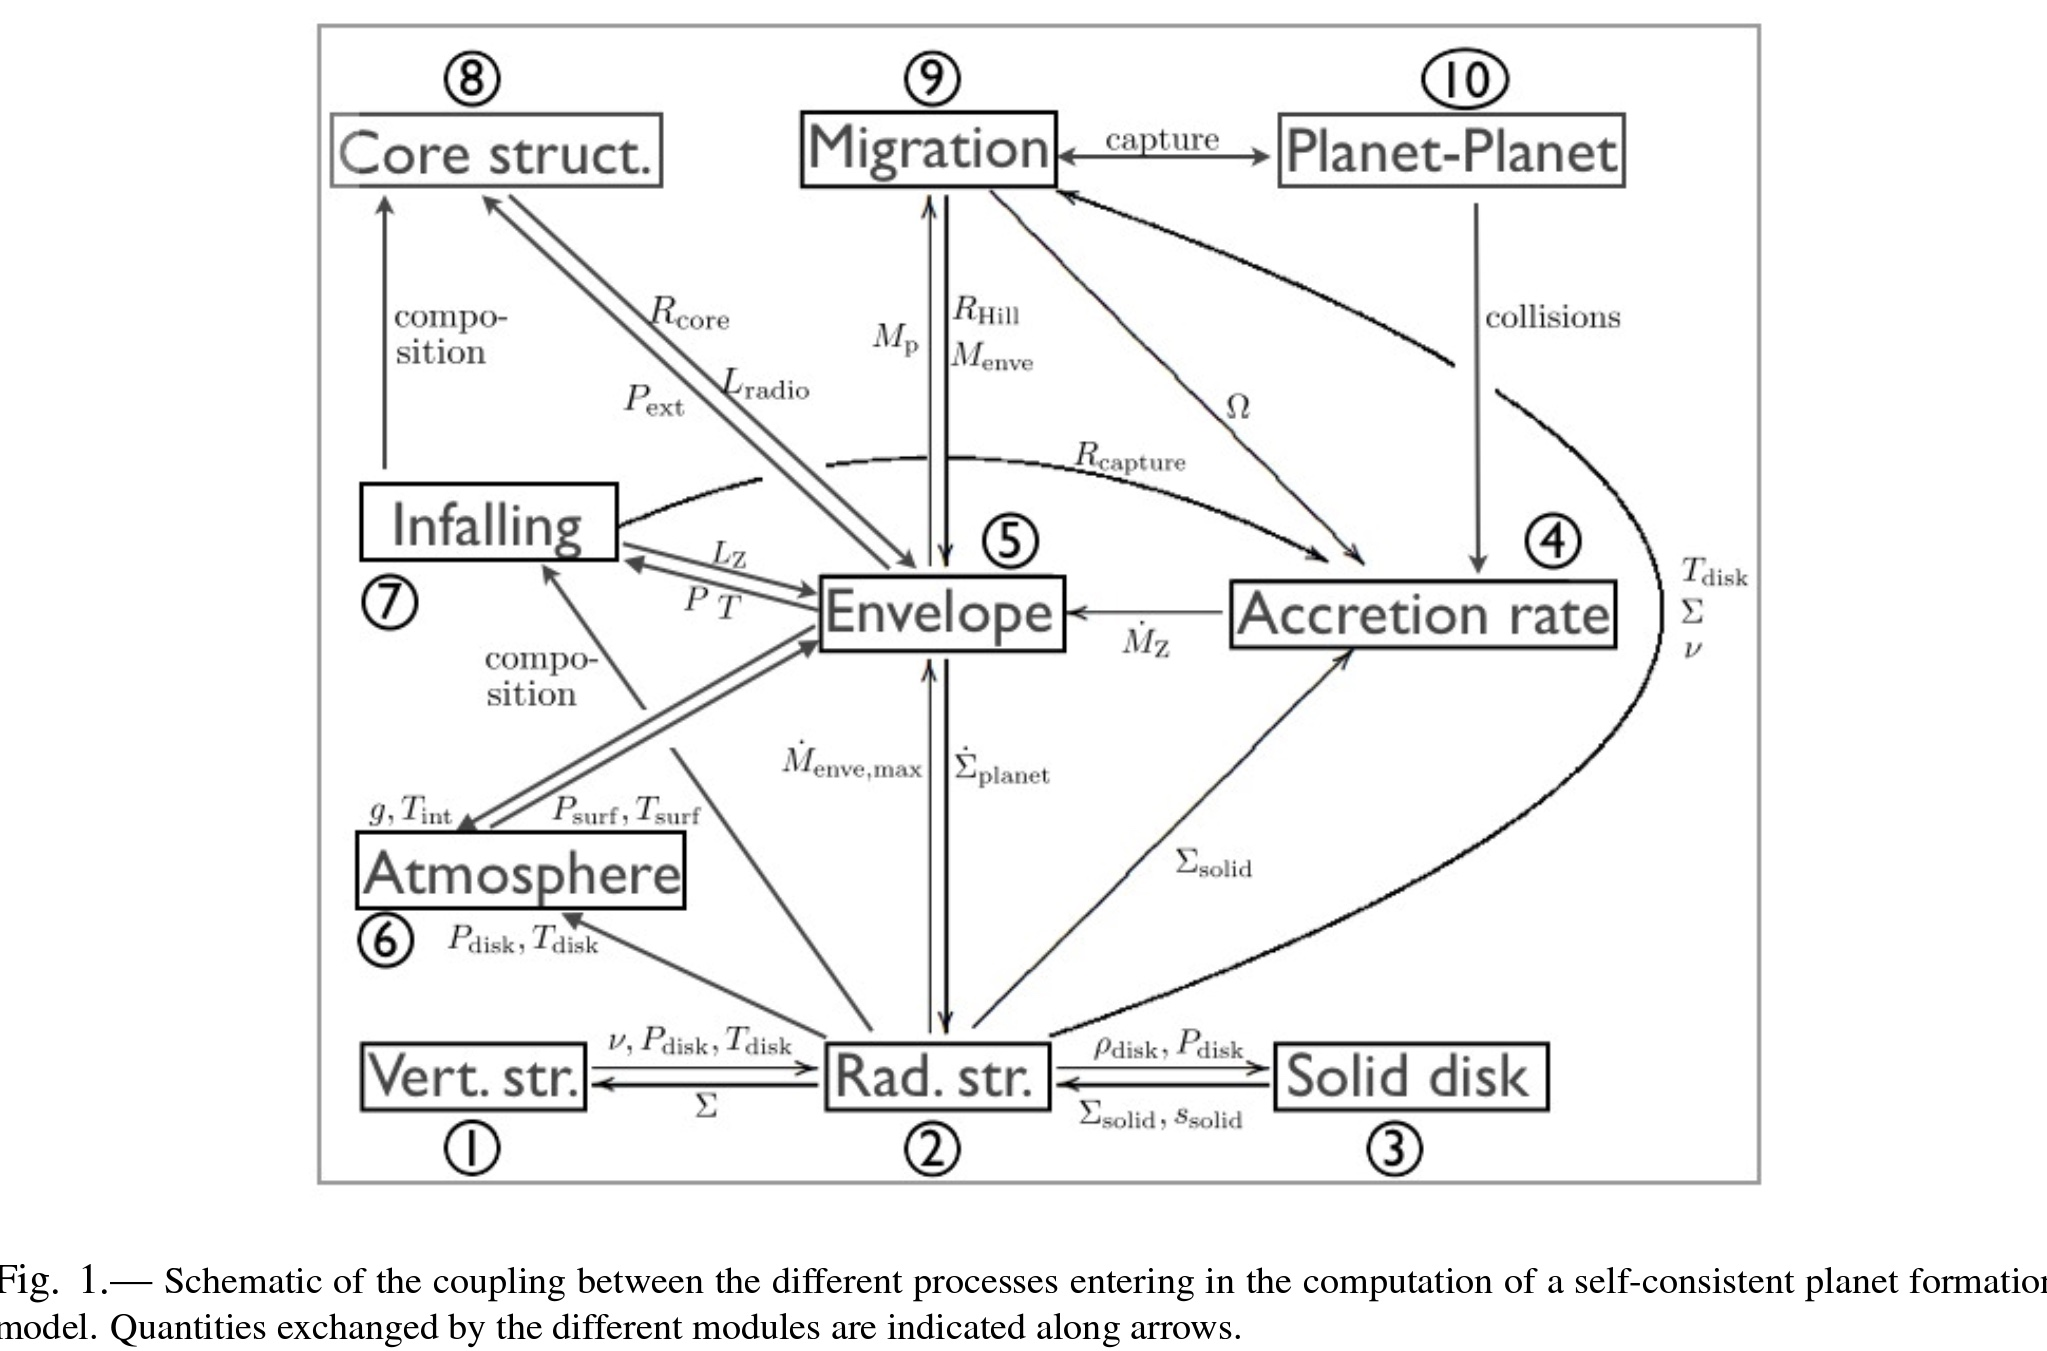
\includegraphics[trim={8cm 5cm 8cm 0},clip, keepaspectratio, width=0.7\textwidth]{GFM}
\caption{Schema dei processi che \'e necessario includere in un modello di formazione planetario coerente.
 Da \cite{benz2014planet}.}\label{fig:GFM}
\end{wrapfigure}

La struttura del disco protoplanetario determina la rapidit\'a di accrescimento degli embrioni planetari  principalmente tramite la densit\'a di polvere, influenzata a sua volta dalla posizione dell'iceline ($H_2O$): \'e possibile tenere traccia della frazione di rocce o ghiacci accrescuti. L'interazione tra disco ed embrione che da luogo alla migrazione \'e determinata dalla struttura del disco e dalla massa del pianeta.

Una volta che il core dell'embrione planetario \'e abbastanza massiccio si forma un inviluppo gassoso che inzialmente si raccorda alle condizioni del disco e alla saturazione della capacit\'a del disco di fornire gas si stacca dal disco: la struttura del pianeta \'e quindi determinata da massa, raggio e luminosit\'a del core, massa gassosa legata al pianeta, energia rilasciata da accrescimento planetesimi e gas.

La capacit\'a del pianeta di accrescere planetesimi aumenta con l'aumentare della massa e del raggio del pianeta.

\begin{errata}[atmosfera e luminosit\'a pianeta: discorsivo]
 Le condizioni in fondo all'atmosfera planetaria forniscono le condizioni di temperatura e pressione all'estremo dell'inviluppo gassoso. La struttura del disco determina anche il rate massimo di accrescimento del gas. Il rate d'accrescimento di solidi \'e determinato dalla sezione d'urto efficace, determinata dalla struttura dell'inviluppo gassoso, dalla densit\'a di solidi nel disco e dalla velocit\'a orbitale. La luminosit\'a del pianeta \'e determinata dal rate di accrescimento dei solidi e dal rate di contrazione del pianeta. Infine la migrazione \'e determinata dalla caretteristiche del disco e dalla massa del pianeta.
\end{errata}

\begin{workout}[Ref PPS]
Towarddeterminist model of planetary formation iV: effectsof type I migration
									: accumulation neare iceline
									: dynamical intaraction and coagulation of multiple rocky embrios (isolation mass, semi-analytic vs n-body)
									: eccentricity distribution of gas giant
Theoretical models of planetary system formation: mass vs. semi-major axis	(alibert carron 13)			Lecture 15 -planetary ...
Modelling planetary system formation with N-body simulation (11)
Global model of planet formation and evolution
Planetary population synthesis
planet population synthesis					
\end{workout}

\section{Modello disco di accrescimento e distribuzione condizioni iniziali}
%Refs: Sec4 mordasini09
%\cleardoublepage

\begin{workout}[planet luminosity]
\begin{align}
&L=L_{cont}+L_{acc}\\
&L_{cont}=-\frac{E_t(t+dt)-E_t(t)-E_{gas,acc}}{dt}\\
&E_{gas,acc}=dt\,\dot{M}_{gas}u_{int}\\
&L_{acc}=G\frac{\dot{M}_{core}M_{core}}{R_{core}}
\end{align}
\end{workout}

Tramite metodi di montecarlo si determinano numerose combinazioni delle condizioni iniziali del disco e dei parametri scelti per descrivere la sua struttura.
Le variabili di montecarlo hanno distribuzione determinata dalle osservazioni.

\begin{workout}[modello globale: evoluzione dal semplice al complesso]
Global model of planets formation and evolution: more detailed submodels
\end{workout}

Il modello pi\'u semplice di disco di accrescimento usa distribuzione esponenziale per andamento densit\'a superficiale e temperature, assumendo disco otticamente sottile, e relazione $L_*\propto M_*^4$ di sequenza principale. Le lacune di questo modello sono
\begin{itemize}
\item i dischi sono otticamente spessi con transizioni nell'opacit\'a
\item non \'e presente evoluzione temporale consistente
\end{itemize}

Modelli pi\'u recenti  risolvono l'equazione per l'evoluzione viscosa:
\begin{align}
&\TDy{t}{\Sigma}=\frac{1}{r}\PDof{r}[3r\expy{1/2}\PDof{r}(\nu\Sigma r\expy{1/2})]+\dot{\Sigma}_w(r)+\dot{\Sigma}_{embryo}(r)\label{eq:diskaccrphev-m18}\\
&\dot{\Sigma}_w(a)=\left\{\begin{array}{c}0\quad a<R_g\\\frac{\dot{M}_w}{2\pi(a_{max}-R_g)a}\quad \text{altrimenti}\\\end{array}\right.
\end{align}
con $\dot{\Sigma}_w$ contributo della foto-evaporazione (\cite{veras2004outward}), $R_g=\SI{5}{\astronomicalunit}$ e $a_{max}$ estremo del disco,  $\dot{\Sigma}_{embryo}$ contributo di accrescimento di gas e componente solida dei pianeti.
La densit\'a superficiale iniziale \'e assunta essere:
\begin{equation}
\Sigma(a,t=0)=\Sigma_0(\frac{r}{1AU})\expy{p_g}\Exp{[-(\frac{r}{R_o})\expy{2+p_g}]}(1-\sqrt{\frac{r}{R_i}})
\end{equation}
dove i parametri possono essere scelti casualmente secondo una distribuzione di probabilit\'a ricavata dalle osservazioni.

La distribuzione di massa e la frazione di dischi protoplanetari per ammassi stellari di et\'a diversa \'e mostrata in figura (\ref{fig:initdistro}). La massa \'e determinata misurando il flusso di emissione termica della polvere: la distribuzione di $\log{M_{disk}}$  \'e gaussiana e per il cluster Ophiuchus la distribuzione \'e fittata da gaussiana corrispondente a massa media $M_{disk}=0.042\msun{}$.

Il tempo caratteristico del disco \'e determinato dalla viscosit\'a $\alpha$: fissata $\alpha$ compatibile con tempo caratteristico osservato $\tau_{disk}^{obs}\approx\SI{3}{\mega\year}$ e assumendo la distribuzione uniforme nel logaritmo di $\dot{M}_w$, si calcola  $t_{disk}(\alpha,\Sigma_0,\dot{M}_w)$ determinando gli estremi dello fotoevaporazione per riprodurre tempi di vita osservati.

Valori tipici sono $\dot{M}_w=\SIrange{5e-10}{3e-8}\msun{}/\si{\year}$ per $\alpha=\num{7e-3}$.

Nelle popolazione planetaria considerata $\alpha$ \'e fissato compatibilmente con le osservazioni  ed \'e omogeneo e costante.

\begin{figure}[!ht]
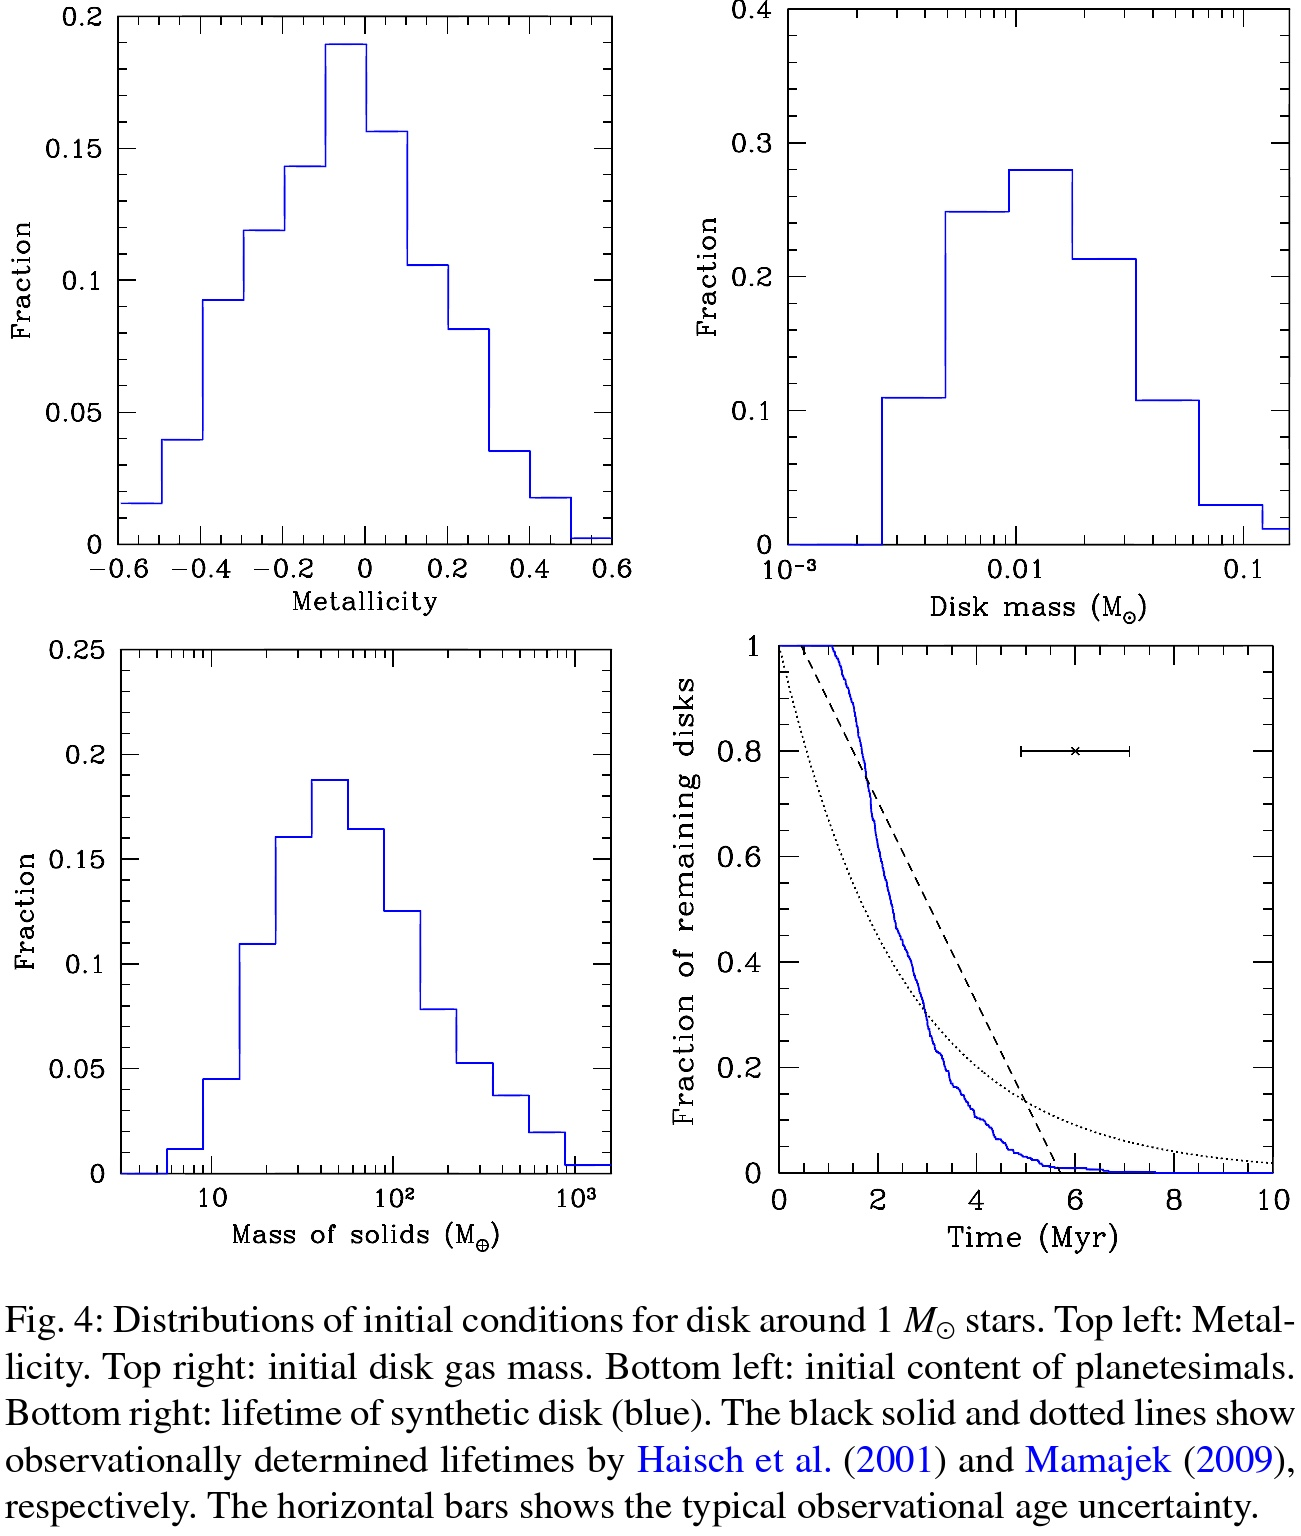
\includegraphics[trim={0cm 10cm 0 0},clip, keepaspectratio,width=0.7\textwidth]{initdistro}
\caption{Distribuzione caretteristiche dischi di accrescimento. Da \cite{mordasini2018planetary}.}\label{fig:initdistro}\end{figure}

\begin{workout}[viscosit\'a disco]
Nella popolazione planetaria simulata $\alpha$ \'e fissato sulla base delle osservazioni  ed \'e omogeneo e costante.
\end{workout}

\begin{workout}[Modello di disco di accrescimento - (Mordasini18: 4) - Introduzione descrizione fenomeni grazie a PPS]
Refs: garaud lin 07, chiang goldreich 97
Un modello di disco  di accrescimento usato nelle simulazioni considera l'evoluzione della densit\'a superficiale tramite l'equazione \eqref{eq:diskaccrphev-m18}
\begin{align}
&\TDy{t}{\Sigma}=\frac{1}{r}\PDof{r}[3r\expy{1/2}\PDof{r}(\nu\Sigma r\expy{1/2})]+\dot{\Sigma}_w(r)+\dot{\Sigma}_p(r)\label{eq:diskaccrphev-m18}\\
&\dot{\Sigma}_w(a)=\left\{\begin{array}{c}0\\\frac{\dot{M}_w}{2\pi(a_{max}-R_g)a}\\\end{array}\right.
\end{align}
Densit\'a superficiale iniziale:
\begin{equation}
\Sigma(a,t=0)=\Sigma_0(\frac{r}{1AU})\expy{p_g}\Exp{[-(\frac{r}{R_o})\expy{2+p_g}]}(1-\sqrt{\frac{r}{R_i}})
\end{equation}
4-Mordasini18 (Hayashi81). $p_g\approx1$ (Andrews10).
\end{workout}

\section{Distribuzione iniziale planetesimi ed evoluzione}

Assumendo conversione completa di polvere in planetesimi, la densit\'a superficiale di planetesimi \'e
\begin{equation}
\Sigma_p(t=0,r)=f_{dg}\eta_{ice}\Sigma_g(t=0,r)
\end{equation}
con $f_{dg}$ rapporto gas/polvere (circa metallicit\'a) \'e una parametro casuale con distribuzione che riflette distribuzione di metallicit\'a stellari, $\eta_{ice}$ tiene conto della discontinuit\'a nella distribuzione superficiale di solidi all'iceline.

Sulla scorta della piccola differenza tra composizione solare e composizione meteoritica e assumendo inoltre che il ferro sia un buon indicatore della componente solida  si usa la formula
\begin{equation}
\frac{f_{D/G}}{f_{D/G\odot}}=10\expy{[\cel{Fe}{}{}{}/\cel{H}{}{}{}]}
\end{equation}
con $f_{D/G\odot}\approx\numrange{0.01}{0.02}$ (\cite{lodders2003solar}).

\begin{workout}[Planet host stars are enriched in nikel and silicon]
Robinson06
\end{workout}

Si introduce un fattore correttivo per il drift della polvere entro i \SI{20}{\astronomicalunit} compreso tra $2-4$ (\cite{kornet2004alternative}) e infine si sfrutta la distribuzione della metallicit\'a per stelle di massa solare nelle vicinanze del Sole:
\begin{equation}
p([Fe/H])=\frac{1}{\sigma\sqrt{2\pi}}\exp{-\frac{([Fe/H]-\mu)^2}{2\sigma^2}}
\end{equation}
Per le stelle campionate da CORALIE (\cite{udry2000coralie}, 1650 stelle nane entro \SI{50}{\parsec}) si ha $\mu=-0.02$ e $\sigma=0.22$.

L'evoluzione della distribuzione dei planetesimi tiene conto dell'acrescimento sugli embrioni planetari
\begin{equation}\dot{\Sigma}_p=-\frac{(3M_*)\expy{1/3}}{6\pi a_p^2B_LM_p\expy{1/3}}\dot{M}_c\end{equation}
e generalmente si assume che eccentricit\'a e inclinazione seguono distribuzione di Rayleigh.

Il drift dei planetesimi dovuto all'interazione col gas e la formaziane gap nella distribuzione dei planetesimi sono di solito trascurati.

\begin{workout}[Initial planetesimal distro]
Dust converted early everywhere fully-efficient (mordasini18: pg 12),Thommes pg8)
\begin{align*}
&\Sigma_p(t=0,r)=f_{dg}\eta_{ice}\Sigma_g(t=0,r)\\
&\dot{\Sigma}_p(r)=-\frac{1}{2\pi aB_LR_H}\dot{M}_c
\end{align*}
Icelines Mordasini 1141: inside where T exceeds sublimation
{Embryo starting position}
Usually a distro uniform in log(a): relative spacing of few Hill spheres (Kokubo Ida 10)
Ida, lin10: asymptotical isolation mass ''Toward a Deterministic Model of Planetary Formation VI'',
Trapped evolution model: Hasegawa pudritz 11, Cridland 16
\end{workout}

\section{Caratteristiche iniziali degli embrioni planetarii e accrescimento}

La massa iniziale dei core deve essere molto minore della massa di isolamento: si usano 20-50 embrioni di frazioni di massa terrestre ($0.01-0.1\mearth{}$); la distanza dalla stella varia seguendo distribuzione di probabilit\'a $p(a)$ inversamente proporzionale alla distanza orbitale $p(a)\,da\propto\frac{da}{\Delta}\propto\,d\log{a}$. Il momento di comparsa \'e determinato dal rate di accrescimento dei planetesimi \eqref{eq:Gaccretionpl}.

La massa dei core varia per l'accrescimento dei planetesimi secondo
\begin{align}
&\dot{M}_c=\Omega\Sigma_pR^2_{capt}F_G
%&\dot{\Sigma}_p(r)=-\frac{1}{2\pi aB_LR_H}\dot{M}_c
\end{align}

Per determinare l'accrescimento di gas \'e necessario calcolare la struttura planetaria in alternativa si pu\'o averne una stima da
\begin{align}
&\dot{M}_{e,KH}=\frac{M_p}{\tau_{KH}}\\
&\tau_{KH}=10\expy{p}(\frac{M_p}{\mearth{}})^q(\frac{\kappa}{\si{\gram\per\square\cm}})\si{\year}
\end{align}
dove p,q sono ottenuti tramite modelli di struttura planetaria; \cite{mordasini2014grain} hanno determinato $\kappa=\SI{e-2}{\gram\per\square\cm}$, $p=10.4$ e $q=-1.5$.

\begin{workout}[Grain opacity and the bulk composition of extrasolar planets (Alibert mordasini klahr)]
$b=10.4+\log{f}$
\end{workout}

\begin{workout}[Higher mass gap formation reduces accretion rate]
\begin{equation}
f_{va04}=1.668(\frac{M_p}{\mjupiter{}})\expy{1/3}\exp{-\frac{M_p}{1.5\mjupiter{}}}+0.04
\end{equation}
\end{workout}


\section{Popolazioni planetarie sintetiche}
%Considero i risulati di alcuni modelli di formazione planetari (\cite{mordasini2018planetary}).
\begin{errata}[Soluzione del modello di formazione globale]
La soluzione del modello di formazione planetario variando le condizioni iniziali in maniera opportuna e determinando un gran numero di combinazioni tramite metodi di montecarlo produce un ensemble di sistemi da cui, tramite confronto statistico con la popolazione osservata, si valuta l'accuratezza delle .
\end{errata}

%\subsection{Progresso nei modelli di formazione globale}

\begin{workout}[Risultati dello sforzo di riprodurre la forma del diagramma a-M]
Alcuni risultati prodotti dal tentavo di migliorare l'accordo tra popolazioni sintetiche  e popolazione pianeti reali:
\begin{itemize}
\item Il modello di migrazione GT80 e tanaka02 producono migrazipone troppo veloce (mordasini09: assenza pianeti minori di 10masse solari entro 0.1AU). L'analisi del momento torcente di corotazione in dischi non isotermi dimostra che questo fenomeno pu\'o essere la soluzione alla migrazione troppo rapida, inoltre si pu\'o avere migrazione verso l'esterno con formazione di zone di convergenza.
\item rate di accrescimento di gas runaway (ida lin 04: deserto di pianeti tra 10-100 masse terrestri): il calore generato dall'accrescimento di pianetesimi ritarda l'accrescimento di gas e nei modelli recenti i a molti embrioni si ha competizione per il gas
%\item Migrazione II: flussi di gas
\item molteplicit\'a: effetti sui pianeti di piaccola massa sono scattering (eccitazione eccentricit\'a o espulsione), cattura in risonanza e collisioni
\item Relazione con massa stellare: Stelle di minor massa sono circondate da dischi di minore massa: quindi minor frequenza di giaganti.%Relazione tra $\eta_J-M_*$
\end{itemize}
\end{workout}

%\subsection{Popolazione M18}

\begin{figure}[!ht]
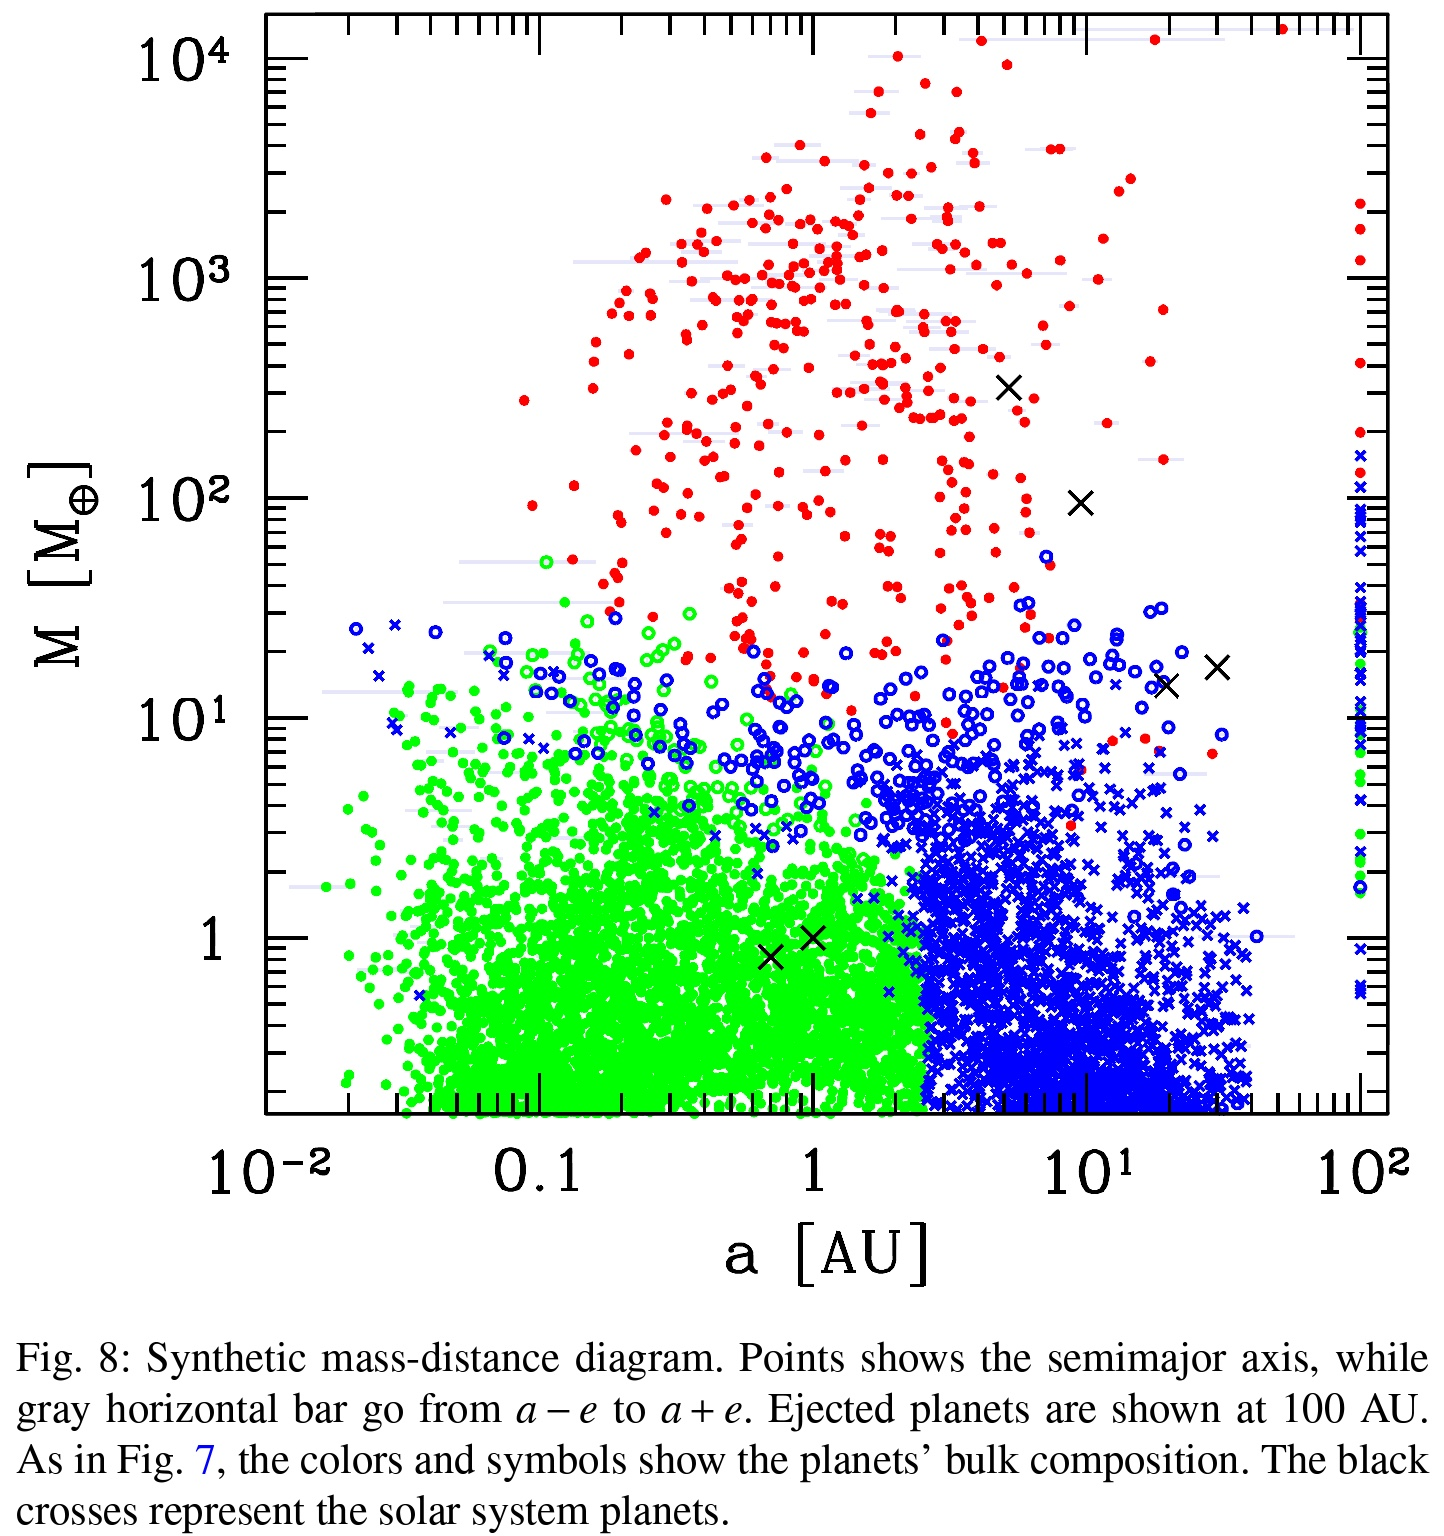
\includegraphics[trim={0cm 8cm 0 0},clip, width=0.9\textwidth,keepaspectratio]{ma-synth}
\caption{Simulazione popolazione planetaria di 504 sistemi Punti rossi: pianeti giganti con $M_e/M_c>1$; simboli blu/verdi: pianeti che hanno accresciuto core con ghiacci/rocce; punti aperti: $0.1\leq M_{env}/M_{core}\leq1$; croci blu e punti pieni verdi: pianeti con $M_{env}/M_{core}\leq0.1$. Da \cite{mordasini2018planetary}.}\label{fig:ma-synth}
\end{figure}

La figura (\ref{fig:ma-synth}) mostra la distribuzione della popolazione sintetica nel diagramma massa-distanza: la posizione finale di un pianeta \'e terminata principalmente dai tempi caratteristici di accrescimento e migrazione; considerando inoltre l'interazione gravitazionale tra i pianeti si hanno effetti delle risonanze e eccitazione di eccentricit\'a.

\begin{figure}[!ht]
\begin{subfigure}[b]{0.47\textwidth}
\centering
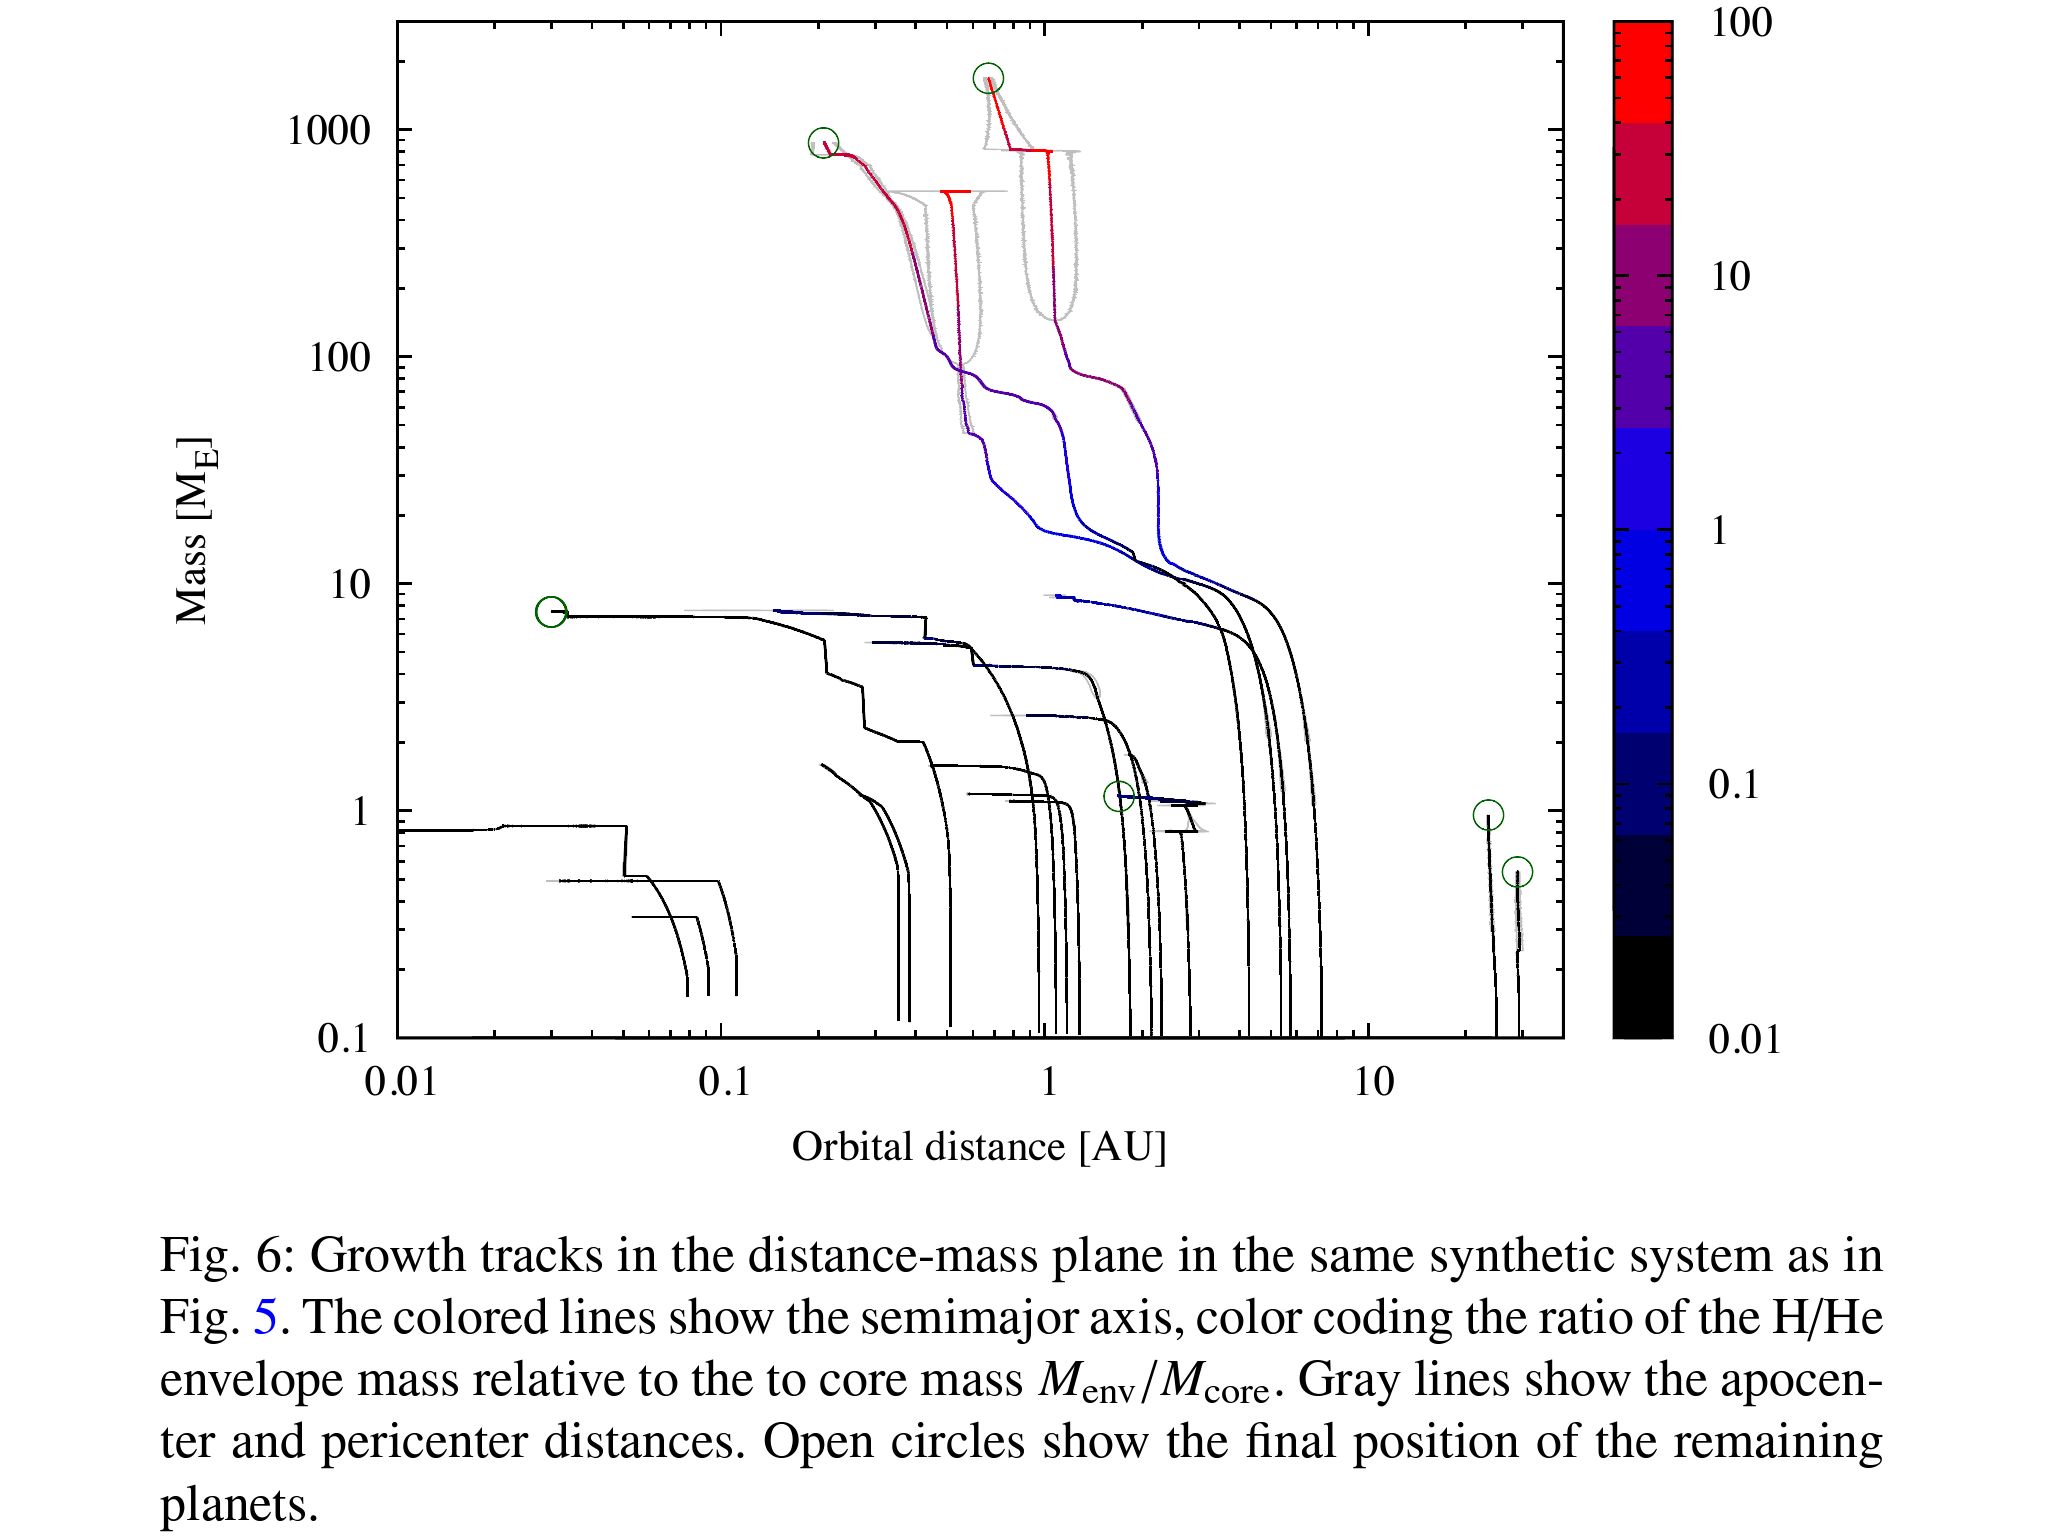
\includegraphics[trim={2cm 12cm 2cm 0},clip, width=\textwidth,keepaspectratio]{track1}
\caption{Formazione di un sistema planetario nel diagramma $a-M$: alla scomparsa del disco protoplanetario si hanno 2 pianeti giganti, un nettuniano caldo e 3 pianeti terrestri. La scala di colore indica la composizione $\frac{M_e}{M_c}$. Da \cite{mordasini2018planetary}.}\label{fig:track1}
\end{subfigure}
~
\begin{subfigure}[b]{0.47\textwidth}
\centering
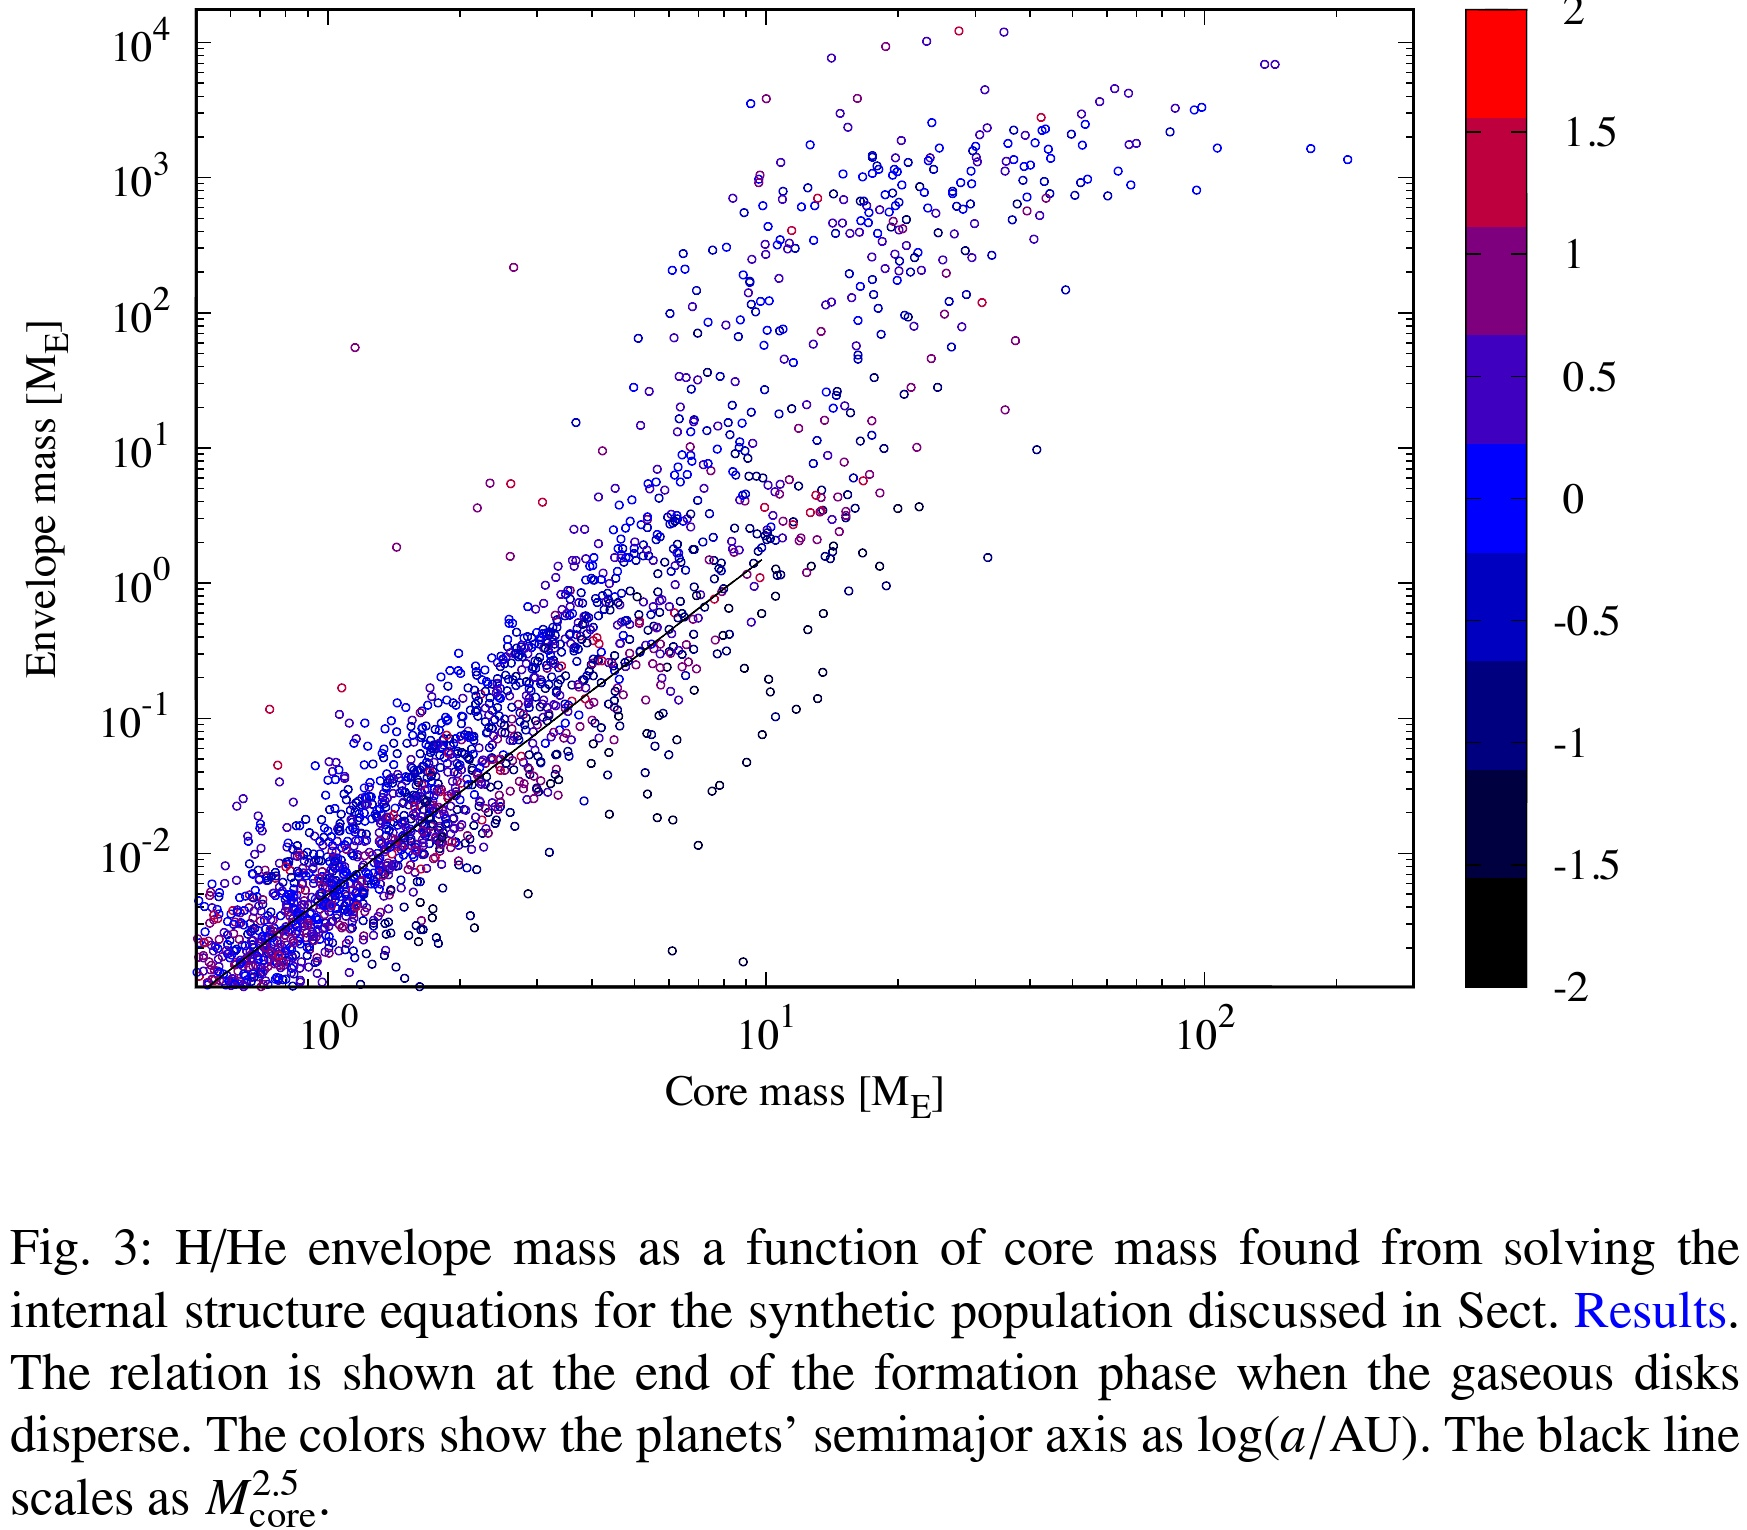
\includegraphics[trim={0cm 12cm 0 0},clip, width=0.9\textwidth,keepaspectratio]{envelopecoresynth}
\caption{Massa inviluppo gassoso vs massa core. Il colore indica la distanza in $\log{\frac{a}{\si{\astronomicalunit}}}$. La linea continua mostra andamento $M_c\expy{-q_{KH}-1}=M_c\expy{2.5}$ precedente alla fase runaway di accrescimento gassoso. Da \cite{mordasini2018planetary}. }\label{fig:envelopecoresynth}
\end{subfigure}
\end{figure}

Alcune caratteristiche dell'ensemble sintetico: %(\cite{mordasini2018planetary}):
\begin{itemize}
\item Numerosi sistemi costituiti da pianeti di piccola massa (\numrange{0.1}{10}$\mearth{}$)
\item Sistemi con pianeti di piccola massa e giganti. Sistemi che mimano il sistema solare con andamento di massa piccolo-massiccio-piccolo (sweet spot per formazione di pianeti giganti \'e all'esterno dell'ice-line).
\item L'architettura dei pianeti giganti varia notevolmente ma quello pi\'u vicino alle stella \'e distanza di circa \SI{1}{\astronomicalunit}, o meno, dalla stella.
\item Piccola percentuale di sistemi con un pianeta gigante superstite di scattering tra pianeti giganti vicini. Sistemi rari formati in dischi massicci con alta metallicit\'a.
%\item Popolazione di pianeti tra $\numrange{30}{100}\mearth{}$: i fattori che influenzano la popolazione di pianeti di massa intermedia sono la massa presente nel disco quando il protopianeta raggiunge la massa critica per accrescimento di gas, il tempo-scala di rilassamento radiativo e competizione per accrescimento di gas tra protopianeti giganti.
\end{itemize}
%saturazione momento di corotazione

Inoltre in figura (\ref{fig:ma-synth}) \'e evidente l'effetto della migrazione rapida all'interno: popolazione pianeti in origine nettuniani (frazione giaccio nel core $50\%$) che migrano all'interno accumulando materiale roccioso (frazione ghiaccio nel core $10-20\%$).

\begin{figure}[!ht]
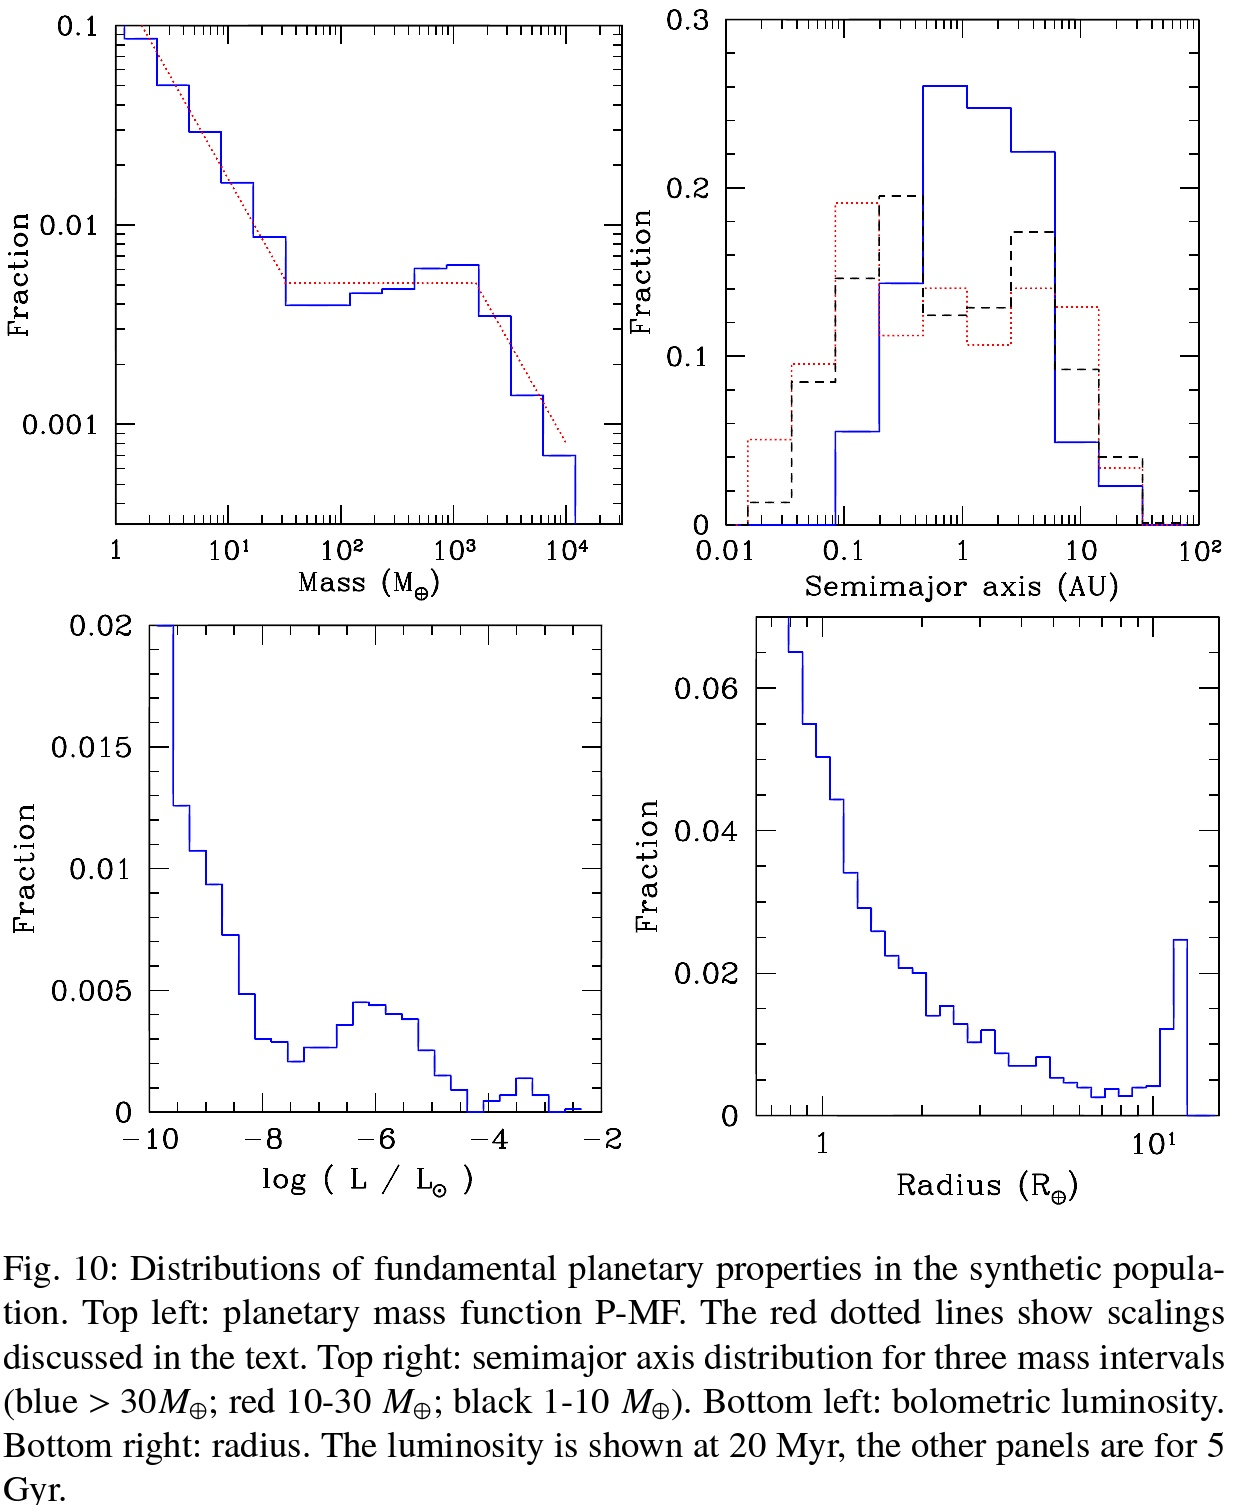
\includegraphics[trim={0cm 10cm 0 0},clip, width=0.9\textwidth,keepaspectratio]{MaLR-freq-synth}
\caption{Distribuzione di massa, semiasse, luminosit\'a, raggio. Da \cite{mordasini2018planetary}. }\label{fig:MaLR-freq-synth}
\end{figure}

\subsection{Caratteristiche delle distribuzioni delle propriet\'a fisiche dei pianeti e significativit\'a}

La figura (\ref{fig:MaLR-freq-synth}) mostra la distribuzione di massa di 509 pianeti della popolazione sintetica di \cite{mordasini2018planetary}. La distribuzione della massa dei pianeti ha andamento diverso per pianeti fino a $30\mearth{}$ formati principalmente da solidi e pianeti che hanno raggiunto la massa critica per l'accrescimento di gas runaway.
%La differente slope della distribuzione di massa nelle due regioni caratterizza i differenti meccanismi di accrescimento.
Si ha un minimo locale attorno alla massa critica dopo di che l'aumento di massa \'e molto veloce verso piccole masse. I risultati sono significativi per masse maggiori delle masse dell'embrione iniziale.

\begin{workout}[Distro luminosit\'a: relazione M-L]
La distribuzione di luminosit\'a segue andamento $L\propto M^2$ con terzo picco per innesco deuterio a $\log{\frac{L}{\lsun}}\approx-3.5$
\end{workout}

La distribuzione del raggio dei pianeti mostra picco a $1\rjupiter$ e crescita per piccoli raggi dovuta al loro lungo $\tkh{}$ e quindi scarso accrescimento di H/He.

La distribuzione dei semi-assi cresce rapidamente tra $0.01-0.1\si{\astronomicalunit}$, resta uniforme in log tra $0.1-10\si{\astronomicalunit}$ nonostante molti pianeti migrino all'interno,mentre i pianeti giganti sono ristretti in \SIrange{0.1}{6}{\astronomicalunit}. La distribuzioni del semiasse non mostra deviazioni dalla distribuzione iniziale.

{\let\clearpage\relax\let\cleardoublepage\relax
\chapter{Confronto semi-quantitativo tra caratteristiche popolazioni sintetiche e osservate}
}

Per confrontare una popolazione planetaria simulata con le osservazioni \'e opportuno, oltre a tenere conto dei bias osservativi, valutare per quali sottoinsiemi dell'ensamble di pianeti ossevati le approssimazioni fatte nel modello sono valide.

\begin{workout}[Relazione $M_p$ vs $Z_p$]
	contenu...
\end{workout}

\begin{workout}[Relazione $Z_*$ metallicit\'a GP]
	contenu...
\end{workout}

\section{Struttura orbitale e tipo di pianeta}

\begin{table}
\begin{tabular}{|ccc|}
\hline
N&Giganti ($M>300\mearth{}$)&vicini ($P\leq100\si{\day}, R\geq\rearth{}$)\\
\hline
1&4.8&8.4\\
2&7.4&12.8\\
3&5.4&11.4\\
4&0.4&10.0\\
$\geq5$&0.0&11.4\\
$\exv{S}$&18.0&54.0\\
O&10-20&50-60\\
\hline
\end{tabular}
\caption{Percentuale di stelle con N pianeti del dato tipo nella popolazione sintetica di \cite{mordasini2018planetary} e confronto con osservazioni.}\label{tab:planetfreq}
\end{table}

La posizione di Nettuno e Saturno nella figura (\ref{fig:ma-synth}) suggerisce che la posizione iniziale fosse probabilmente pi\'u interna (Grand-tack scenario).

La tabella (\ref{tab:planetfreq}) mostra un buon accordo tra teoria e osservazione per frequenza di pianeti giganti e sistemi compatti.

Il confronto della distribuzione di massa tra teorica e osservata mostra il buon accordo della pendenza nei due regimi di accrescimento e della posizione della massa critica. Per quanto riguarda la distribuzione dei raggi planetarii il picco a $1\rjupiter{}$ \'e meno pronunciato perch\'e sono inclusi solo pianeti giganti vicini e la distribuzione sintetica cresce meno rapidamente a piccoli raggi. Infine il gran numero di pianeti terrestri della popolazione sintetica pu\'o collidere dando luogo a pianeti pi\'u massicci tuttavia le interazioni dinamiche sono simulate solo per il tempo di vita del disco.

\begin{figure}[!ht]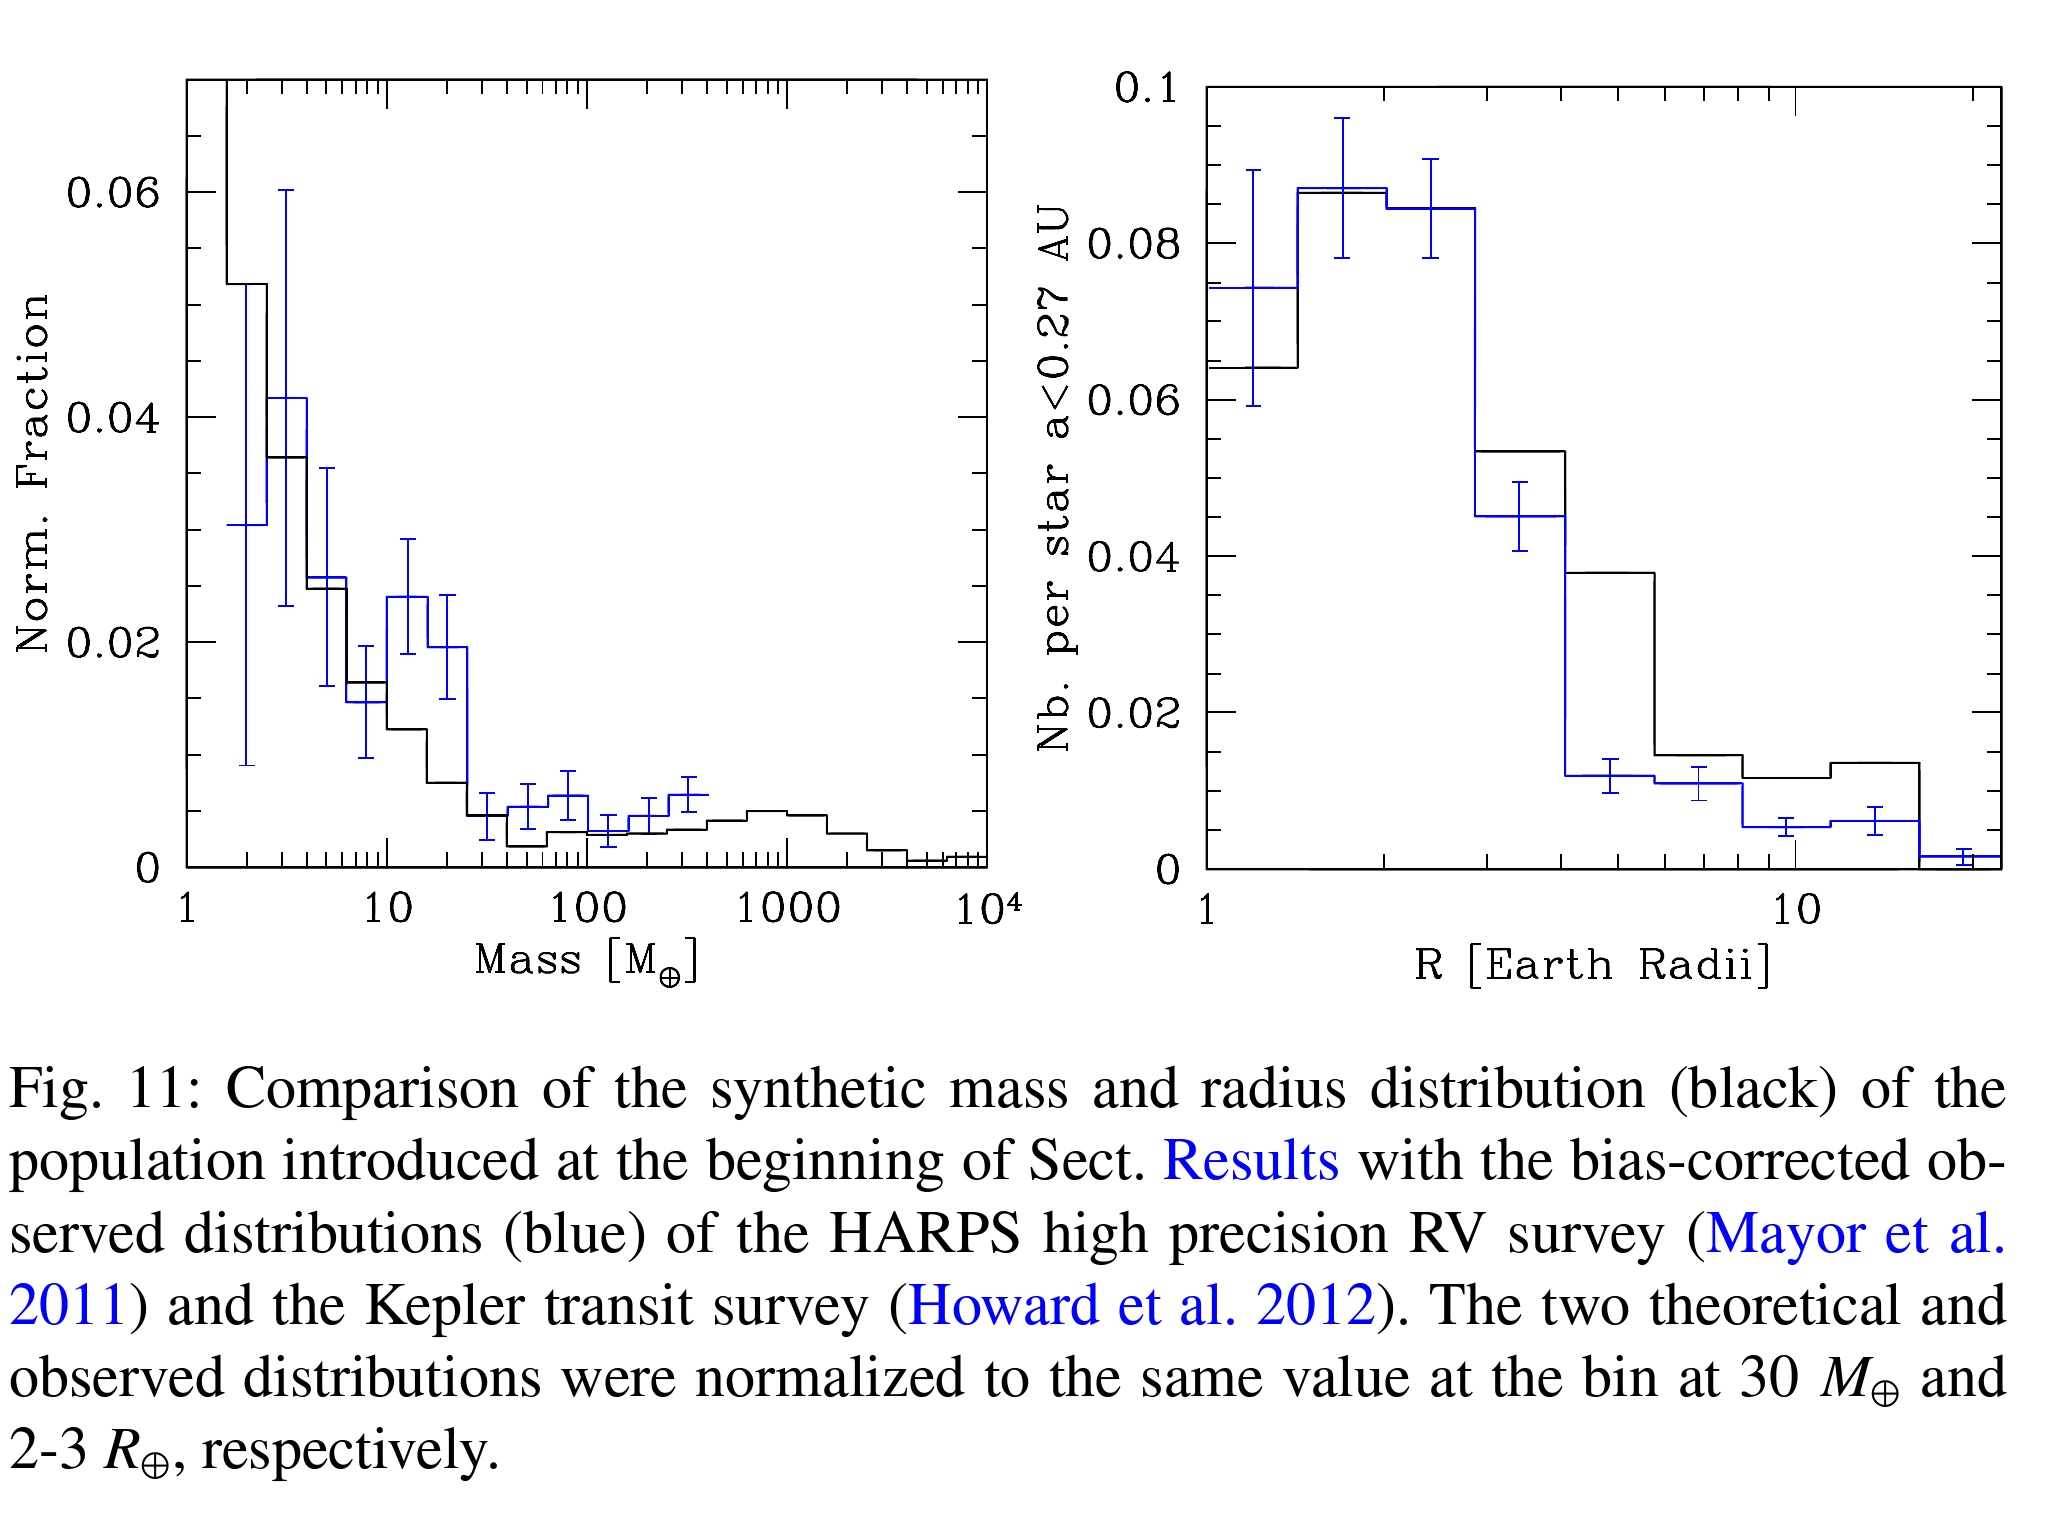
\includegraphics[trim={0cm 17cm 0 0},clip, keepaspectratio,width=0.9\textwidth]{MR-freq-obssynth}\caption{Distribuzioni di massa e raggio per popolazione planetaria sintetica (linea nera) e distribuzioni osservate tramite RV e transiti (linea blu) corrette per i bias. Da \cite{mordasini2018planetary}.}\label{fig:MR-freq-obssynth}\end{figure}

La probabilit\'a di osservare pianeti giganti aumenta con la metallicit\'a: la figura (\ref{fig:giant-Zsynth}) mostra che l'incremento relativo \'e in accordo con le osservazioni.

\begin{figure}[!ht]
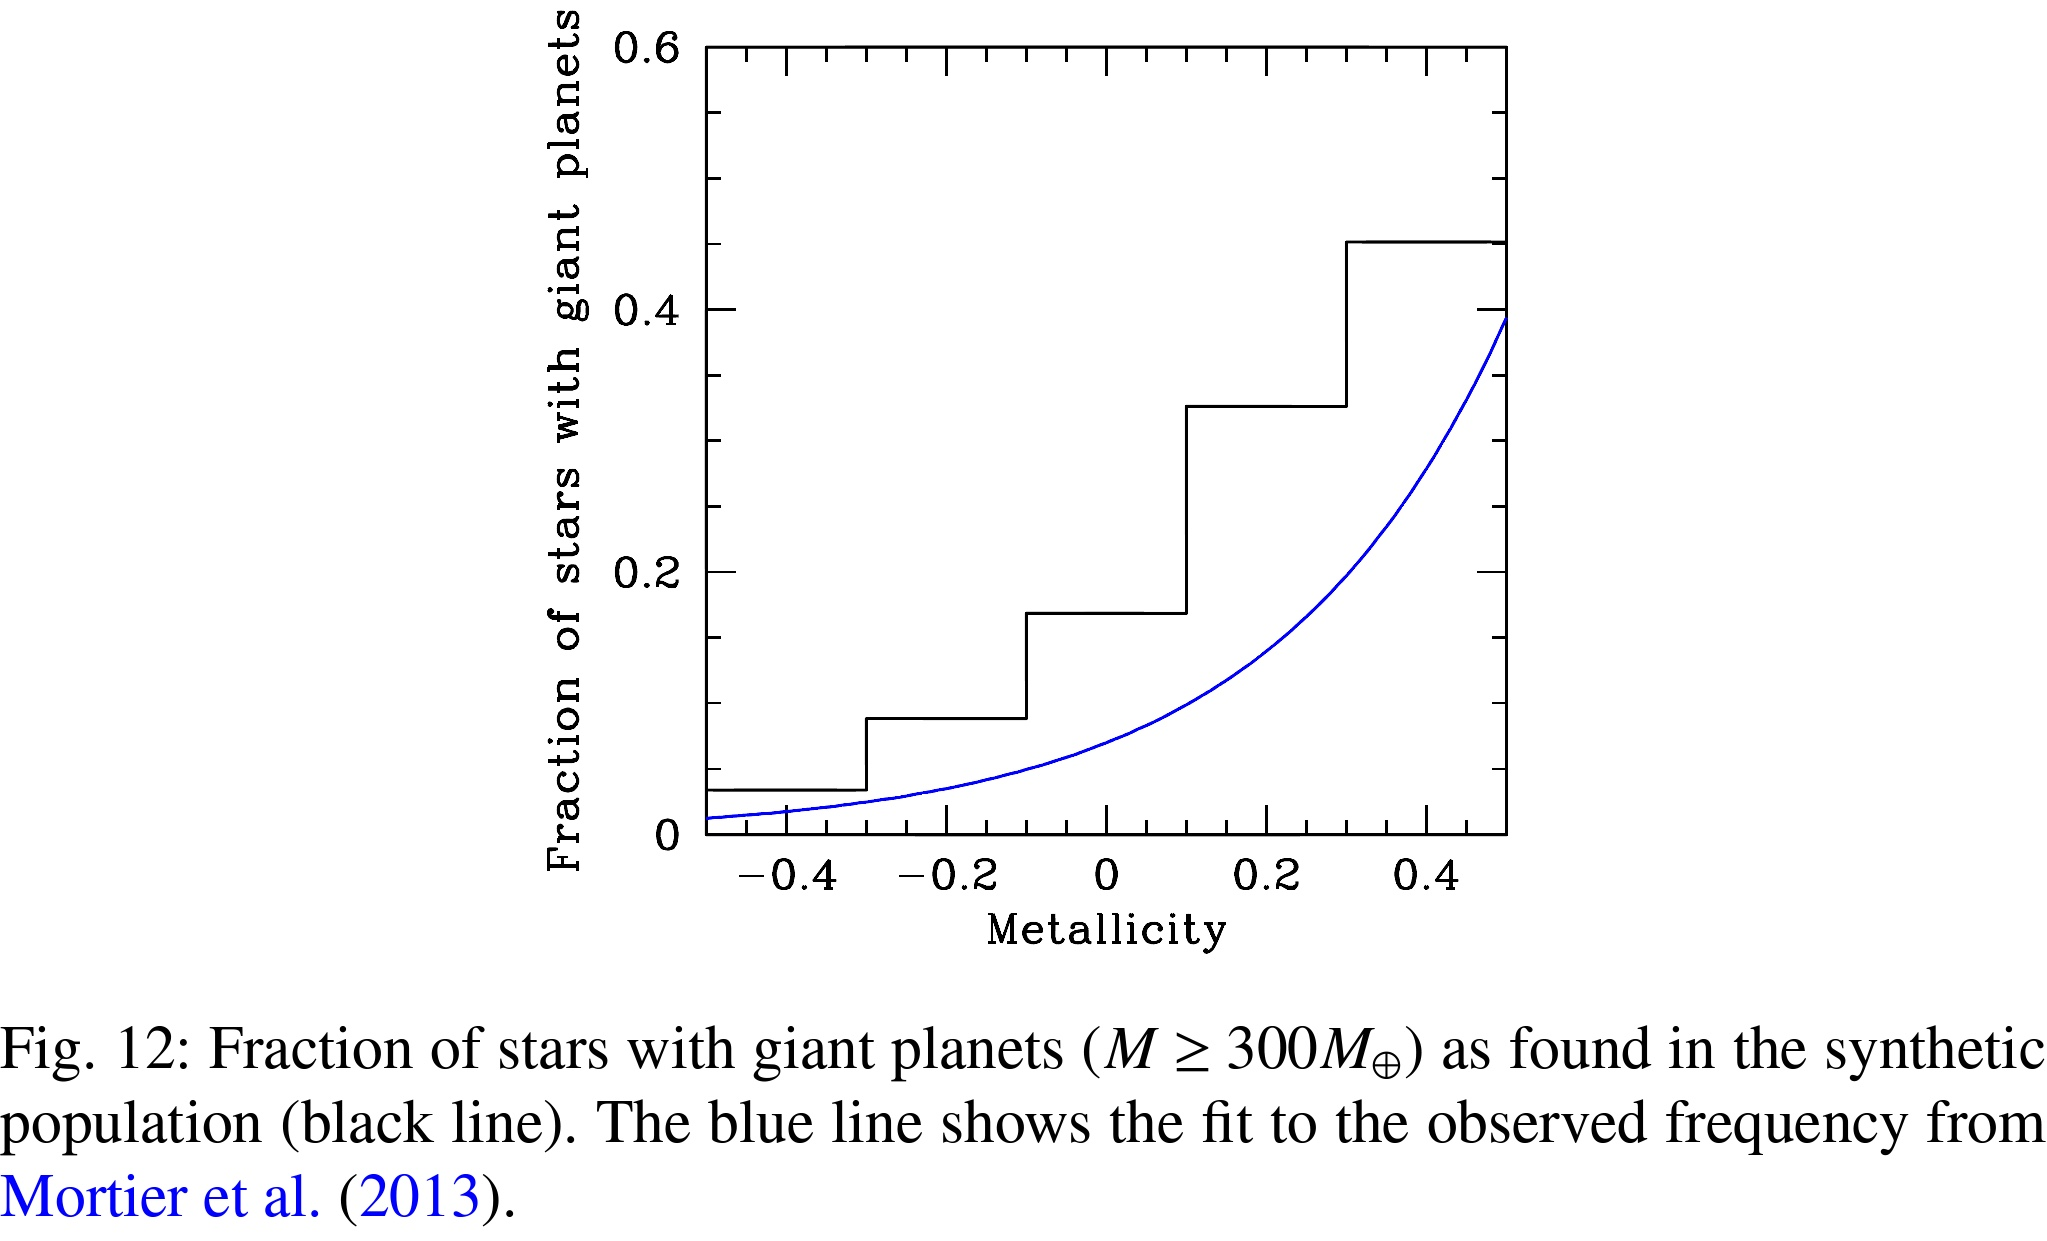
\includegraphics[trim={0cm 10cm 0 0},clip, width=0.9\textwidth,keepaspectratio]{giant-Zsynth}
\caption{Distribuzione di stelle che ospitano pianeti giganti ($M\geq300\mearth{}$) in funzione della metallicit\'a. Nero: popolazione sintetica. Blu: fit da osservazioni. Da \cite{mordasini2018planetary}. }\label{fig:giant-Zsynth}
\end{figure}

\begin{workout}[Orbital structure and MMR: comparison simulation/observation]

\end{workout}

\begin{workout}[Comparison with stellar initial mass function]
Stelalr imf: chabrier 03, salpeter slope 1955
\end{workout}


%{\let\clearpage\relax\let\cleardoublepage\relax
%\chapter{Raffinamento dei modelli}
%}


\begin{workout}[Effects of saturation, cooling and irradiation.]
Impact of planet migration model on planetary populations: effects of saturation, cooling and stellar irradiation (??)
Outward migration helps some planets to become massive, accumulation zone at certain semiaxis, at what mass corotation saturate?
Migration of protoplanets in radiative disks
\end{workout}
